% -*- TeX -*- -*- FR -*-
\documentclass[francais,letterpaper]{uds-article}

%-----------------------------------------------------------------------------
%----- Identification des packages n�cessaires
%-----------------------------------------------------------------------------

\usepackage{babel}
\usepackage[latin1]{inputenc}
%\usepackage{udstitle,dfd}
%\newcommand{\diamant}{Diamant}
\setlength{\oddsidemargin}{0.25in}
\setlength{\evensidemargin}{0.25in}
\setlength{\textwidth}{6.0in}
%\setlength{\parskip}{0.2in}
\newcounter{auxcounter}
\renewcommand{\baselinestretch}{1.5}
\setlength{\parskip}{1.5ex plus0.5ex minus0ex}

\newcommand{\ints}{\renewcommand{\baselinestretch}{1.0}\small \normalsize}
\newcommand{\intm}{\renewcommand{\baselinestretch}{1.5}\small \normalsize}
\newcommand{\intd}{\renewcommand{\baselinestretch}{2.0}\small \normalsize}

\newcommand{\bi}{\begin{itemize}}
\newcommand{\ei}{\end{itemize}}
\newcommand{\be}{\begin{enumerate}}
\newcommand{\ee}{\end{enumerate}}
\newcommand{\bd}{\begin{description}}
\newcommand{\ed}{\end{description}}



\newcommand{\bv}{\verb}

\newcommand{\bve}{\verb*}

\newcommand{\brun}{\noindent $\triangleright$}
\newcommand{\erun}{$\triangleleft$}

\newcommand{\ang}{\textsf}
\newcommand{\key}{\textsf}
\newcommand{\ita}{\textit}
\newcommand{\bld}{\textbf}
\newcommand{\dos}{\textsc}
\newcommand{\pro}{\texttt}

\newcommand{\diamant}{DIAMANT}
\newcommand{\dia}{DIAMANT 1.0}
\newcommand{\dx}{DIAMANT 1.5}
\newcommand{\saphir}{SAPHIR}
\newcommand{\sig}{SIG}

%-----------------------------------------------------------------------------
%----- Page Titre
%-----------------------------------------------------------------------------

\Titre{DX\\
Manuel utilisateur\\
\dx{}}
\Logo{Images/logoDX.eps}
\Auteurs{Ruben Gonzalez-Rubio, \\
Yannick Syam\\}
 \Date{\today}

%-----------------------------------------------------------------------------
%----- Identification des fichiers des pages pr�liminaires et bibliographique
%-----------------------------------------------------------------------------

\FichierResume{}
\FichierRemerciements{}
\FichierGlossaire{} % \FichierLexique est �quivalent
\FichiersBibliographie{udsplain}{Inputs/bibDiamant,Inputs/bib2}

%-----------------------------------------------------------------------------
%----- Le document
%-----------------------------------------------------------------------------

\includeonly{UserManualInputs/intro,UserManualInputs/menus,UserManualInputs/horaire}

\begin{document}
\begin{articleDX}

\chapter{Introduction}


    \section{But}

    \diamant{} est un logiciel servant � la construction d'horaires de
    cours et d'examens sur plusieurs sites � partir d'une interface
    utilisateur.

    \section{Conventions propres � ce document}

    Les anglicismes devront �tre en italique.

    \section{Auditoire cibl� et suggestions de lecture}

    Ce document s'adresse � toutes les personnes impliqu�es dans le
    d�veloppement de \diamant{} tout au long de son cycle de vie: il
    s'agit des utilisateurs, des analystes, des architectes, des
    concepteurs, des testeurs et du chef de projet.

    \section{�tendu du projet}

    \diamant{} est un logiciel de construction d'horaires pr�sent� aux
    utilisateurs sous forme de fen�tre avec une barre de menus,
    contenant des sous-menus. La fen�tre principale pr�sente une
    grille d�crivant l'horaire sur lequel l'utilisateur travaille. En
    dessous de la grille horaire se trouve une barre de t�ches
    \corrpascal{Est-ce une barre de ``t�che'' ou une barre de
    ``statut'' ?}  montrant les ressources en utilisation (�tudiants,
    enseignants, activit�s et locaux) et les conflits d�tect�s.

    Les sous-menus sont de deux types~: ceux qui d�clenchent
    l'ex�cution d'une fonctionnalit� et ceux qui appellent une bo�te
    de dialogue, puis d�clenchent des actions. En g�n�ral ces menus
    entra�nent une mise � jour des donn�es en fonction du traitement
    d�clench�.


    \section{R�f�rences}

    Manuel d'utilisation de \diamant{}. 
\chapter{Construction d'un horaire avec \dx{}}

Construire un horaire avec \dx{} laisse supposer que l'utilisateur
a d�j� sur son ordinateur les fichiers n�cessaires (ceux du STI et
ceux de la Facult�)~: cours.sig, choixet.sig, disprof.sig et
locaux.txt. Ces fichiers peuvent porter n'importe quel nom, mais
pour notre exemple, les noms sont bien explicites. Il est
conseill� de regrouper toutes les informations concernant les
horaires d'un trimestre dans un r�pertoire (par exemple hiver04 ou
h2004). Ainsi, les fichiers d'importation et les fichiers produits
pendant la construction d'un horaire seront ensemble.

La construction d'un nouvel horaire avec \dx{} comporte trois principales �tapes. Elle d�bute par une
phase de pr�paration (phase 1), se poursuit par une phase de modification et d'�puration des donn�es (phase 2) et se termine par la construction � proprement parler (phase 3). La construction de l'horaire peut se poursuivre au del� de la phase 3, par l'utilisation d'outils permettant de raffiner l'horaire (Affectation manuelle, rapports, etc).

Nous vous pr�senterons dans ce chapitre les phases de
pr�paration d'un horaire avec \dx{}, de modification et d'�puration des donn�es, les
caract�ristiques particuli�res de la construction d'un horaire de
cours et d'un horaire d'examen, et nous terminerons les outils de raffinement de l'horaire. Toutefois, les options du logiciel ne seront pas toutes pr�sent�es.

\section{Production d'un horaire de cours}

\subsection{Pr�paration de l'horaire}\label{finprepa}

\begin{enumerate}
    \item Lancer \dx{}.
    \item Aller au menu \textbf{\emph{Fichier}},
    puis s�lectionner le menu \textbf{\emph{Nouvel horaire}}
    et enfin s�lectionner le sous-menu \textbf{\emph{Horaire cycle}}.
    Une bo�te de dialogue comme celle
de la Figure \ref{selectgrillecyc} doit appara�tre et elle vous
permettra de choisir le fichier (fichier avec extension \emph{.xml})
contenant la d�finition de votre grille horaire.

    \begin{figure}[h]
    % Requires \usepackage{graphicx}
    \begin{center}
        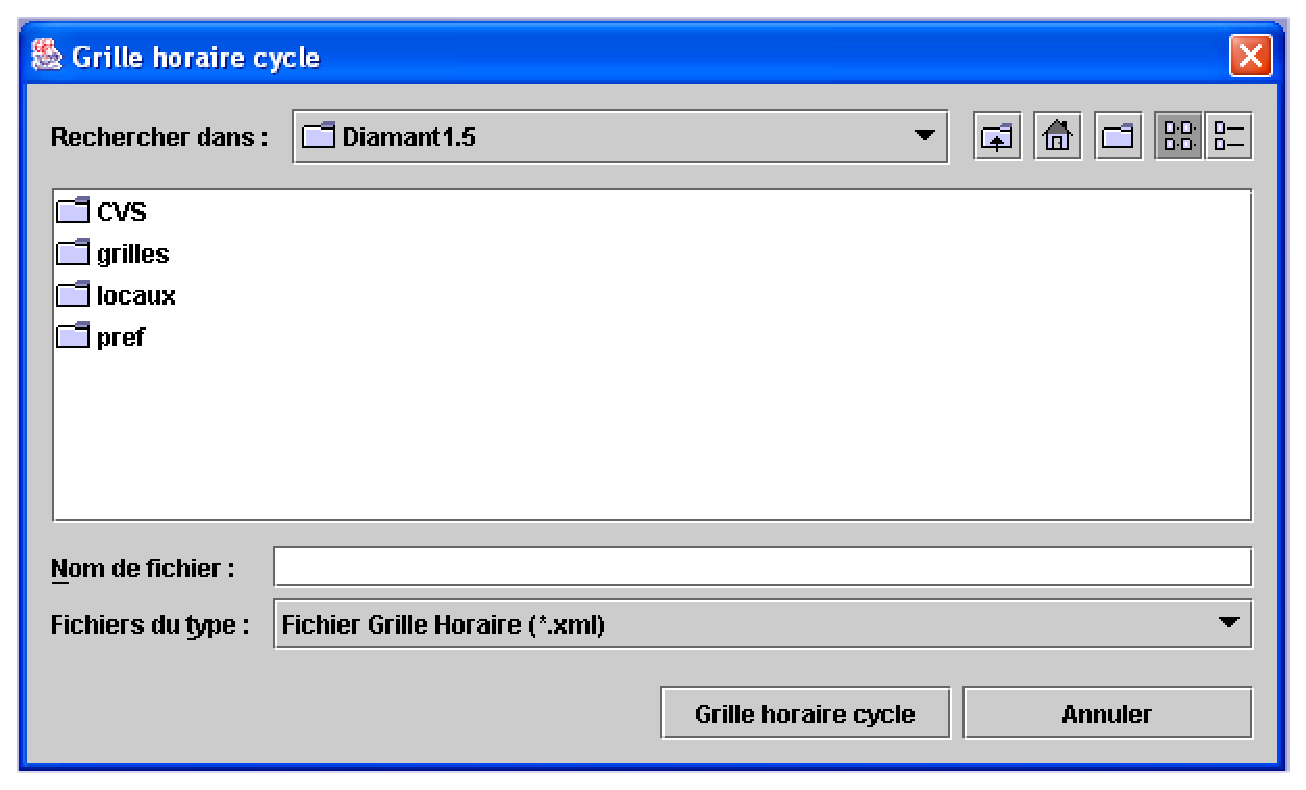
\includegraphics[width=2.5in]{UserManualInputs/images/selectXMLfile.eps}
        \caption{Selection de la grille horaire de cours}\label{selectgrillecyc}
    \end{center}
    \end{figure}

    \item En cliquant sur le bouton \emph{\textbf{OK}}, la grille horaire s�lectionn�e est charg�e et pr�sent�e � l'�cran (voir figure \ref{grillecyc}).
\begin{figure}[h]
  % Requires \usepackage{graphicx}
  \begin{center}
    \includegraphics[width=4.5in]{UserManualInputs/images/grille.eps}
    \caption{Grille horaire de cours}\label{grillecyc}
  \end{center}
\end{figure}

    \item Aller au menu \textbf{\emph{Fichier}} et s�lectionner le menu \textbf{\emph{D�finir fichiers � importer}}. Une bo�te de dialogue comme celle de la Figure \ref{defautoimport}  doit appara�tre. Rep�rer l'endroit o� chacun des fichiers est localis�, puis cliquer sur le bouton \textbf{\emph{OK}}. Une nouvelle fen�tre se pr�sentera afin de vous permettre d'enregistrer la configuration des fichiers que vous venez de faire.

Il est recommand� d'enregistrer cette configuration en utilisant un nom de fichier unique et repr�sentatif.

Exemple: choisissez le nom de fichier \emph{E02cours} pour \emph{�t� 2002 horaire de cours} et le fichier cr�� sera \emph{E02cours.dim}. L'extension \textbf{\emph{.dim}} est rajout� automatiquement.

\begin{figure}[h]
  % Requires \usepackage{graphicx}
  \begin{center}
    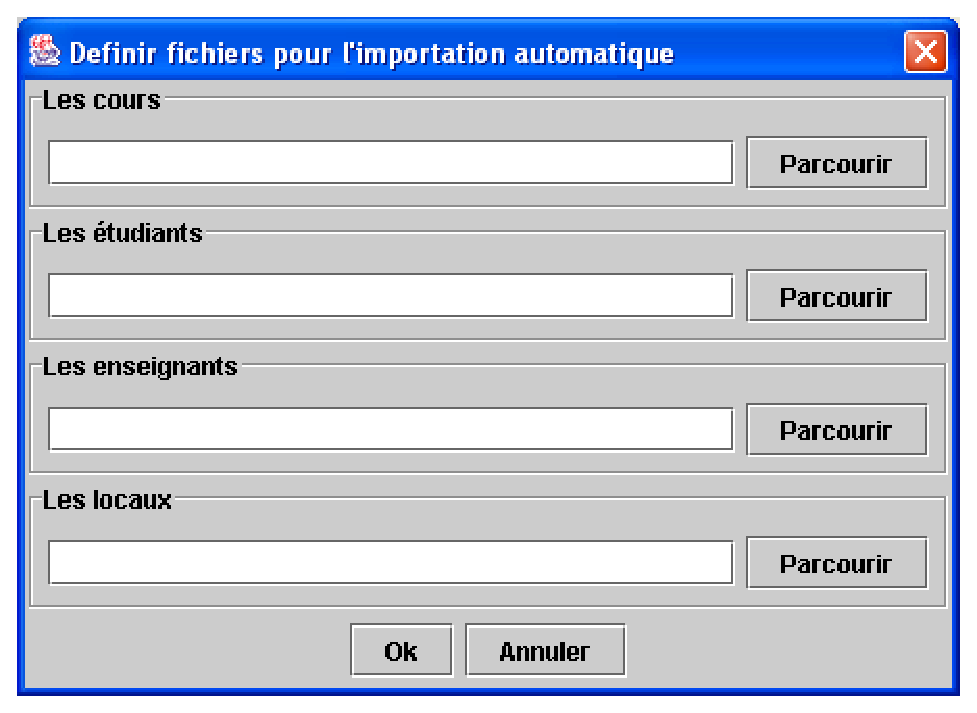
\includegraphics[width=2.5in]{UserManualInputs/images/autoimport.eps}
    \caption{D�finition des fichiers d'importation}\label{defautoimport}
  \end{center}
\end{figure}

    \item Aller au menu \textbf{\emph{Fichier}} et s�lectionner le menu \textbf{\emph{Importer automatiquement}}.
    Une boite de dialogue appara�tra et vous permettra de choisir le fichier \textbf{\emph{.dim}} de �configuration de fichiers�
    pr�c�demment cr�� � partir de la fonction  \textbf{\emph{D�finir fichiers � importer}}
    (dans l'exemple pr�c�dent il s'agit du fichier \emph{E02cours.dim}).
    Cliquer � pr�sent sur le bouton \textbf{\emph{Importation de fichiers}},
    toutes vos donn�es (cours, �tudiants, enseignants et locaux) seront charg�es dans le logiciel et
    pr�tes � �tre modifi�es.
\end{enumerate}

� partir de cette �tape, la construction de l'horaire � proprement parler peut commencer. Il est vivement recommand� de lancer l'\textbf{\emph{affectation initiale}} � partir du menu \textbf{\emph{Optimisation}} avant de poursuivre la production de l'horaire. Lancer l'\textbf{\emph{affectation initiale}} � cette �tape ex�cuterait les fonctionnalit�s suivantes:

\begin{enumerate}
    \item Placer de fa�on al�atoire dans les groupes d'activit�, les �tudiants non pr�-affect�s � des groupes, tout en �quilibrant les groupes.
    \item Placer les �v�nements pr�-affect�s (plac�s ou fig�s) dans la grille horaire.
    \item Calculer les conflits g�n�r�s.
\end{enumerate}

Cette affectation initiale permettrait donc d'initialiser le logiciel de sorte � pouvoir faire des modifications sur les donn�es et observer imm�diatement les repercussions sur l'horaire.

La pr�paration de l'horaire �tant achev�e, nous pouvons � pr�sent passer � la phase de modification et d'�puration de donn�es (phase 2). Il est cependant n�cessaire de noter que cette phase peut avoir lieu avant ou apr�s la phase de construction � proprement parler (phase 3), mais nous recommandons de la faire avant la phase 3 afin de travailler une bonne fois pour toute sur des donn�es propres (�pur�es).

\subsection{Modification et �purations des donn�es}

Le but de cette �tape est de permettre de construire l'horaire uniquement � partir de donn�es propres. Cette modification et/ou �puration peut se faire sur les activit�s, les �v�nements, les groupes d'�tudiants, les enseignants ou les locaux. 

\begin{itemize}
    \item Modifier une activit� en cliquant sur le menu \textbf{\emph{Affectation}} et le sous menu \textbf{\emph{Activit�s}} pour voir appara�tre la \emph{liste des activit�s} (voir figure \ref{listactc}) ou alors cliquer sur le menu \textbf{\emph{Affectation}} et le sous menu \textbf{\emph{�v�nements}} pour voir appara�tre la \emph{liste des �v�nements} (voir figure \ref{listeeventc}).\\

� partir de la fen�tre \emph{liste des �v�nements}, vous pouvez s�lectionner un ou plusieurs �v�nements et les faire passer de la colonne \emph{fig�s} (les �v�nements sont plac�es et fig�es dans la grille horaire) � \emph{plac�s} (les �v�nements sont plac�es dans la grille horaire) ou de la colonne \emph{plac�s} � \emph{non plac�s} (les �v�nements ne sont pas encore plac�es dans la grille horaire) et vice-versa. 

    \begin{figure}[h]
      % Requires \usepackage{graphicx}
      \begin{center}
        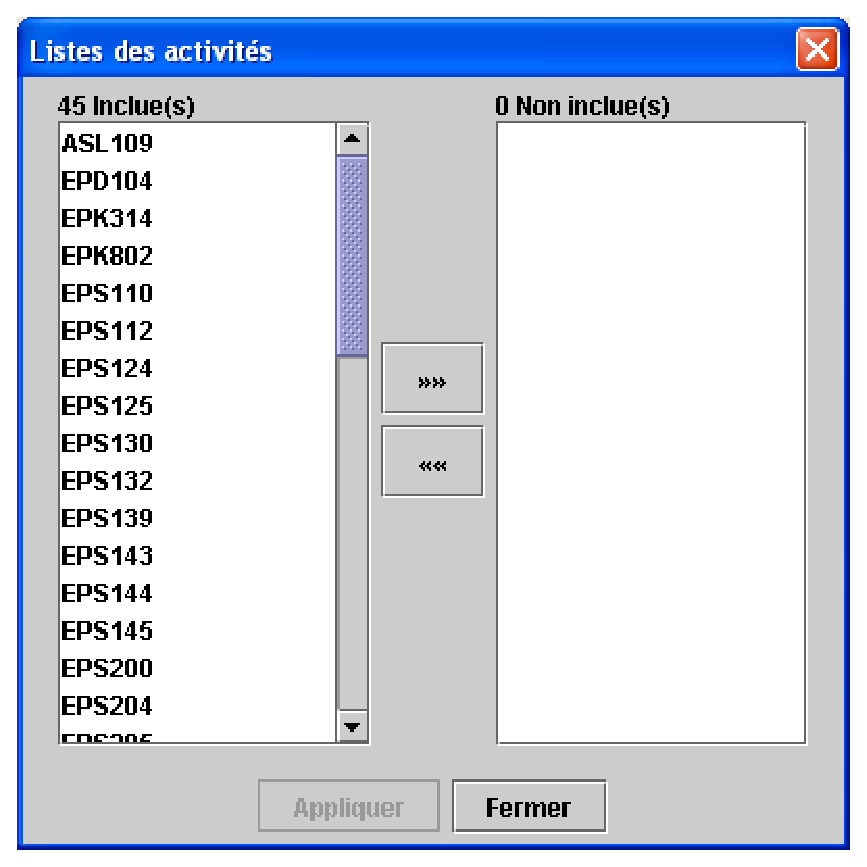
\includegraphics[width=2.5in]{UserManualInputs/images/listeact.eps}
        \caption{Liste des activit�s}\label{listactc}
      \end{center}
    \end{figure}

� partir de la fen�tre \emph{liste des activit�s}, vous pouvez s�lectionner une ou plusieurs activit�s et les faire passer de la colonne \emph{inclue(s)} � \emph{non inclue(s)} (non inclue(s)= les activit�s ne seront pas utilis�es dans la construction de l'horaire) et vice-versa. \\

    \begin{figure}[h]
      % Requires \usepackage{graphicx}
      \begin{center}
        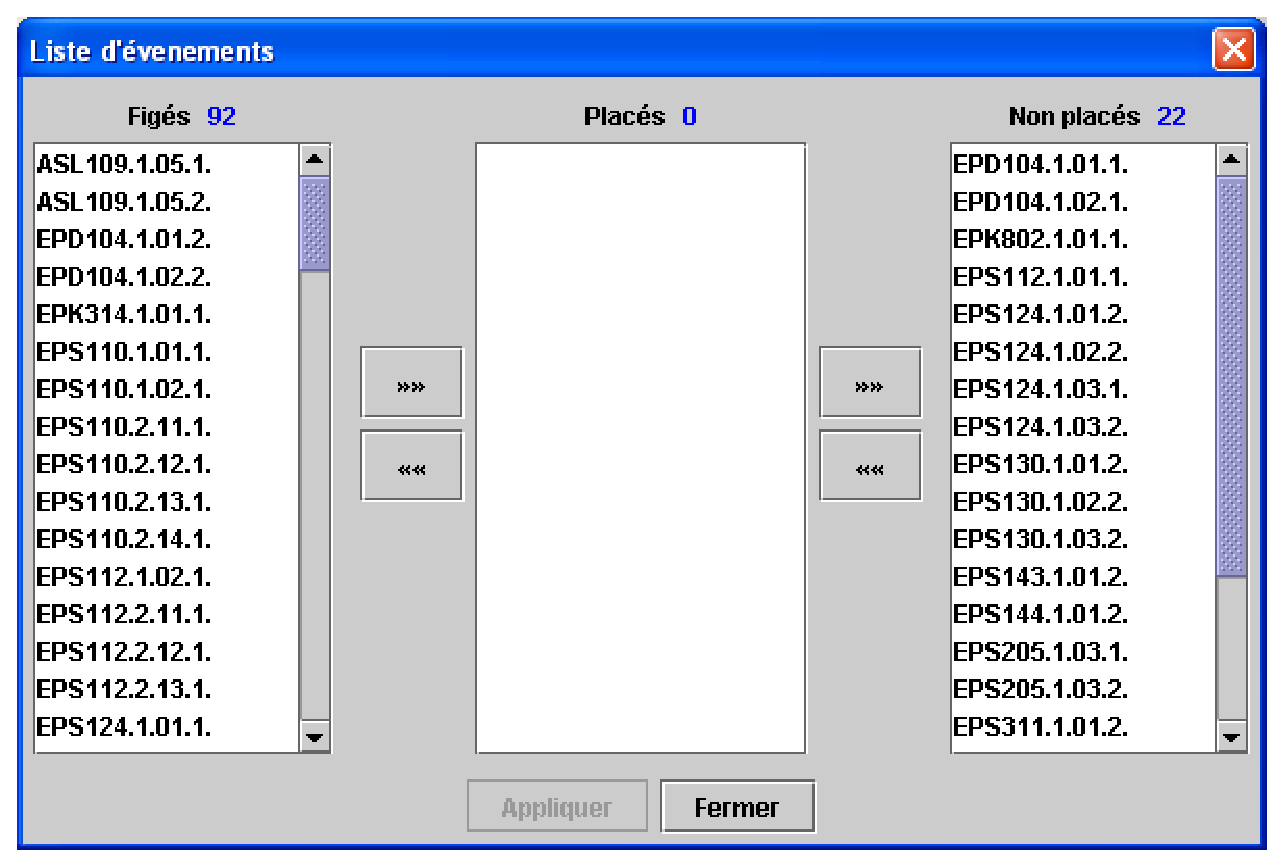
\includegraphics[width=2.5in]{UserManualInputs/images/listeevent.eps}
        \caption{Liste des �v�nements}\label{listeeventc}
      \end{center}
    \end{figure}
   

� partir de l'une ou l'autre des fen�tres, double-cliquer sur l'activit� ou l'�v�nement � modifier pour faire appara�tre le dialogue d'\emph{affectation d'�v�nements} (voir figure \ref{eventc}). Il vous est possible de modifier, � partir de cette fen�tre d'\emph{affectation d'�v�nements}, le jour et l'heure de d�but de l'�v�nement, l'enseignant, le local, de placer ou figer l'activit�.

    \begin{figure}[h]
      % Requires \usepackage{graphicx}
      \begin{center}
        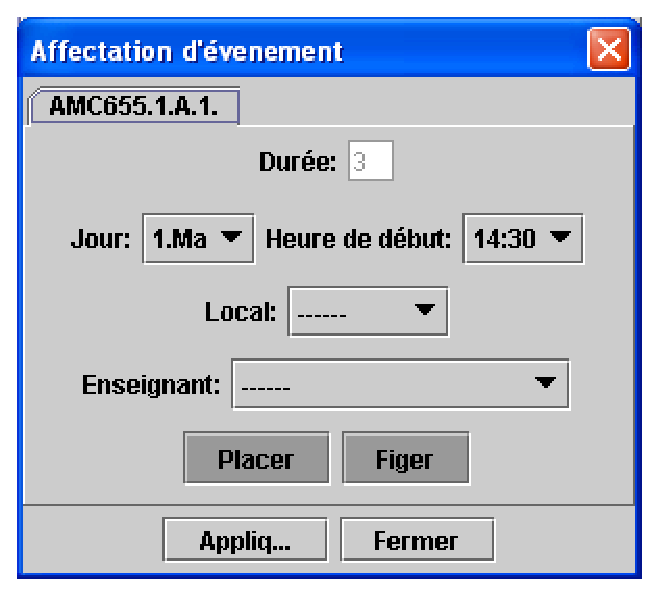
\includegraphics[width=2.5in]{UserManualInputs/images/event.eps}
        \caption{Affectation d'�v�nement}\label{eventc}
      \end{center}
    \end{figure}
    
Cliquer sur \textbf{\emph{Appliquer}} pour valider les changements et Cliquer sur \textbf{\emph{Fermer}} pour fermer la fen�tre.\\
    
    \item Ajouter ou supprimer un groupe ou un �v�nement en cliquant sur le menu \textbf{\emph{Modification}} et le sous menu \textbf{\emph{Activit�}} pour voir appara�tre la fen�tre d'\textbf{\emph{Activit�s}} de la figure \ref{modifactc}.

    \begin{figure}[h]
      % Requires \usepackage{graphicx}
      \begin{center}
        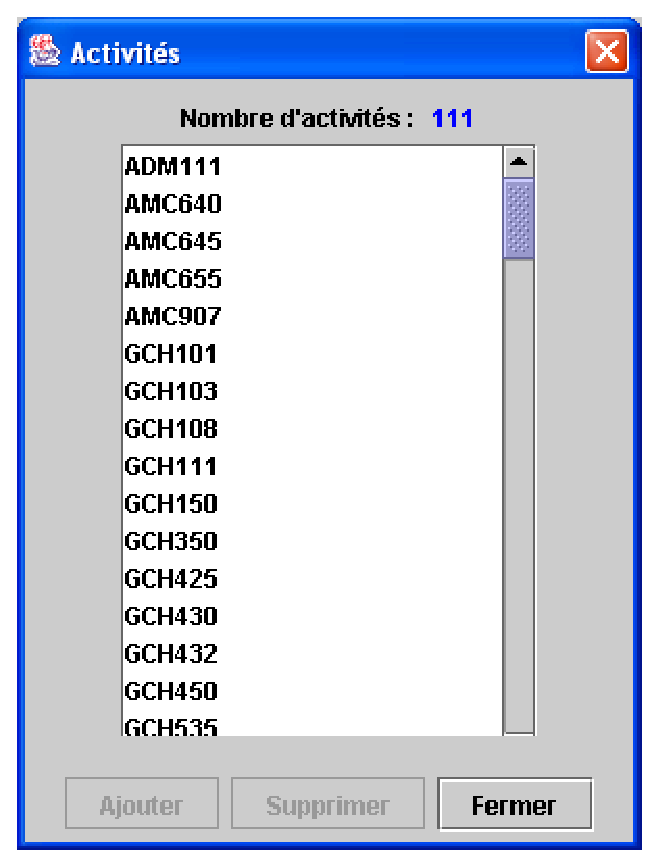
\includegraphics[width=2.5in]{UserManualInputs/images/modifact.eps}
        \caption{Modification d'activit�s}\label{modifactc}
      \end{center}
    \end{figure}

Double-cliquer sur l'activit� que vous souhaitez modifier pour voir appara�tre la fen�tre de \textbf{\emph{Natures}} de la figure \ref{modiftypec}.

    \begin{figure}[h]
      % Requires \usepackage{graphicx}
      \begin{center}
        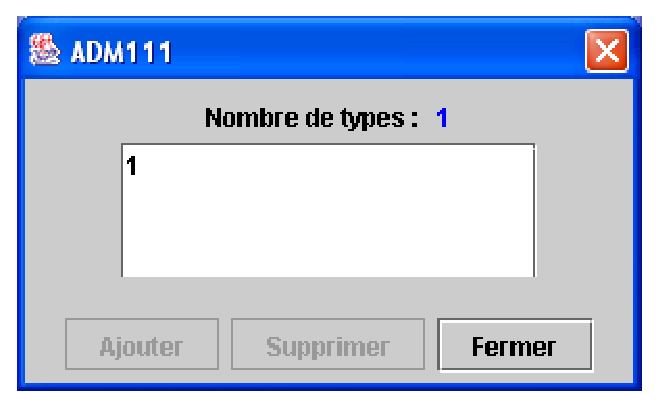
\includegraphics[width=2.5in]{UserManualInputs/images/modiftype.eps}
        \caption{Modification de natures}\label{modiftypec}
      \end{center}
    \end{figure}

Double-cliquer sur la nature que vous souhaitez modifier pour voir appara�tre la fen�tre de \textbf{\emph{Groupes)}} de la figure \ref{modifgroupec}.

    \begin{figure}[h]
      % Requires \usepackage{graphicx}
      \begin{center}
        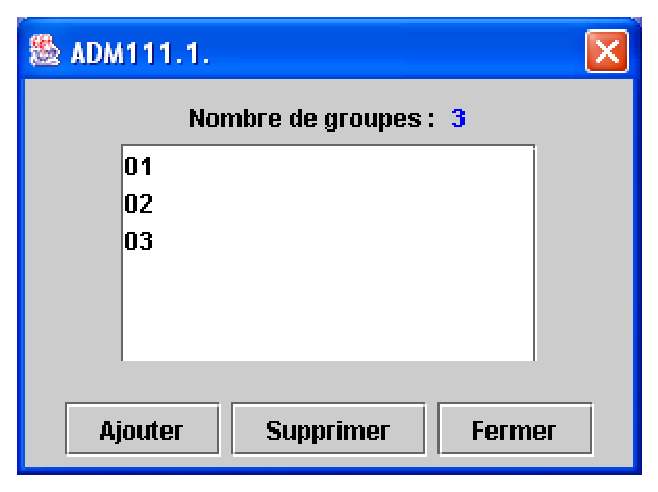
\includegraphics[width=2.5in]{UserManualInputs/images/modifgroupe.eps}
        \caption{Modification de groupe}\label{modifgroupec}
      \end{center}
    \end{figure}
� partir de cette fen�tre, vous avez trois possibilit�s:
        \begin{enumerate}
            \item Cliquer sur le bouton \textbf{\emph{Ajouter}}, pour ajouter un groupe. Le groupe sera ajout� � la suite du dernier groupe de la liste.
            \item Cliquer sur le bouton \textbf{\emph{Supprimer}}, pour supprimer un groupe. Le dernier groupe de la liste sera supprim�.
            \item Double-cliquer sur le groupe que vous souhaitez modifier pour voir appara�tre la fen�tre d'\textbf{\emph{�v�nements}} de la figure \ref{modifunitc}. � partir de cette fen�tre, pour pouvez ajouter, supprimer ou modifier un �v�nement.

    \begin{figure}[h]
      % Requires \usepackage{graphicx}
      \begin{center}
        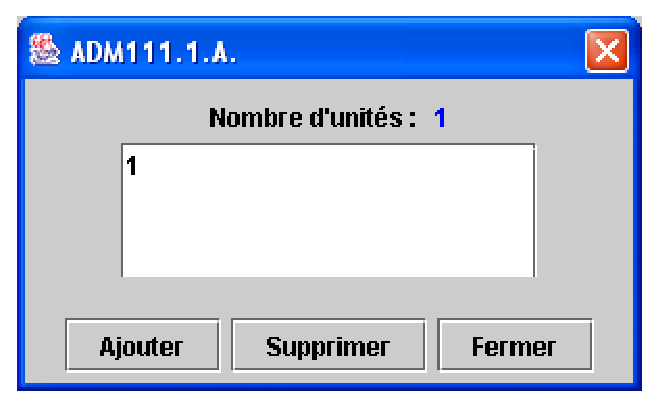
\includegraphics[width=2.5in]{UserManualInputs/images/modifunit.eps}
        \caption{Modification d'�v�nements}\label{modifunitc}
      \end{center}
    \end{figure}
            
            Double-cliquer sur l'�v�nement que vous souhaitez modifier pour voir appara�tre la fen�tre d'\emph{affectation d'�v�nements} (voir figure \ref{eventc}). Il sera possible de faire, dans cette fen�tre, toutes les modifications d�crites pr�c�demment; il �galement possible de modifier la dur�e d'un �v�nement.
        \end{enumerate}    

\item Modifier les groupes d'�tudiants en cliquant sur le menu \textbf{\emph{Affectation}} et le sous menu \textbf{\emph{Groupes}} pour voir appara�tre la fen�tre de la figure \ref{groupec}. S�lectionner dans la colonne de droite (�tudiants assign�s) le groupe (Groupe A, Groupe B, ...) que l'on souhaite modifier. S�lectionner ensuite un ou plusieurs �tudiants que l'on souhaite d�placer. Utilisez enfin les fl�ches pour d�placer les �tudiants de la gauche vers la droite ou vice-versa.

    \begin{figure}[h]
      % Requires \usepackage{graphicx}
      \begin{center}
        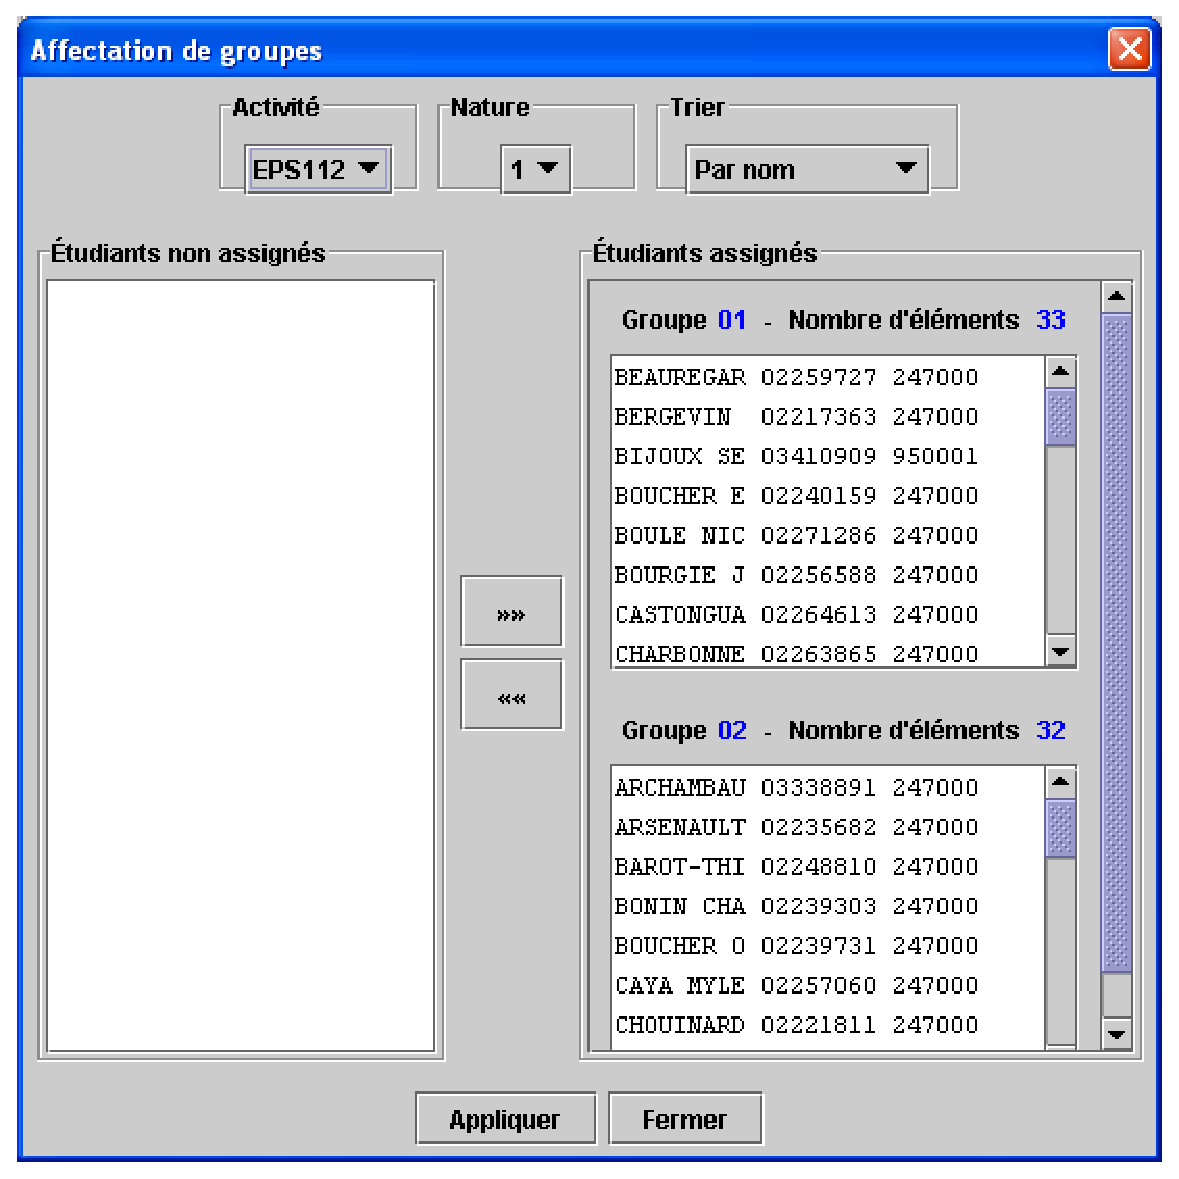
\includegraphics[width=2.5in]{UserManualInputs/images/groupe.eps}
        \caption{Affectation des groupes}\label{groupec}
      \end{center}
    \end{figure}

Cliquer sur le bouton \textbf{\emph{Par matricule/Par programme/Par nom}} dans le zone \emph{trier}, pour trier les �tudiants par matricule, par programme ou par nom.

Cliquer sur \textbf{\emph{Appliquer}} pour valider les changements et Cliquer sur \textbf{\emph{Ok}} pour valider les changements et fermer la fen�tre.\\

\item Modifier la disponibilit� d'un enseignant en cliquant sur le menu \textbf{\emph{Affectation}} et le sous menu \textbf{\emph{Enseignants}} pour voir appara�tre la fen�tre de la figure \ref{enseignantc}. En s�lectionnant une zone correspondant au jour et � l'heure que vous souhaitez modifier. Une zone s�lectionn�e appara�t en fonc� et indique que l'enseignant y est disponible.
 
    \begin{figure}[h]
      % Requires \usepackage{graphicx}
      \begin{center}
        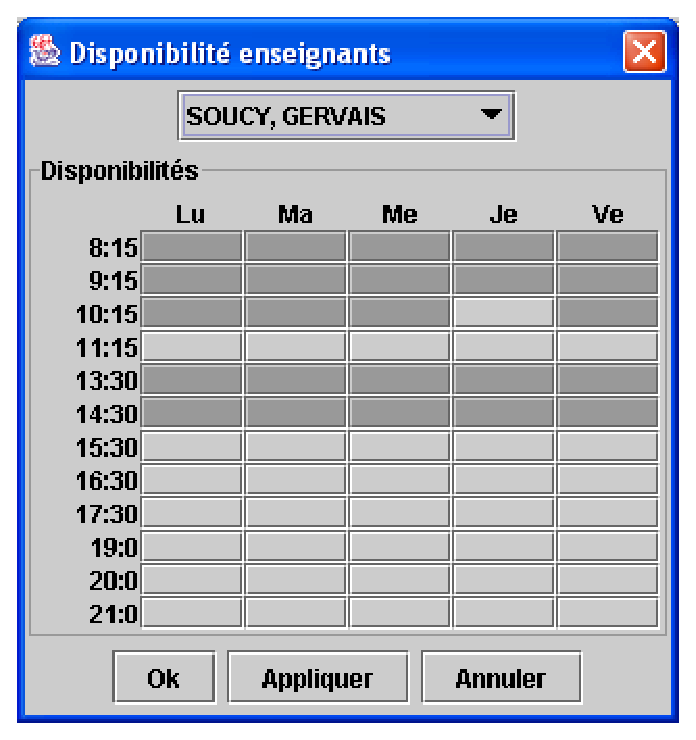
\includegraphics[width=2.5in]{UserManualInputs/images/enseignant.eps}
        \caption{Disponibilit� des enseignants}\label{enseignantc}
      \end{center}
    \end{figure}

Cliquer sur \textbf{\emph{Appliquer}} pour accepter et effectuer les changements et Cliquer sur \textbf{\emph{Ok}} pour accepter, effectuer les changements et fermer la fen�tre.    \\

    \item Modifier la disponibilit� d'un local en cliquant sur le menu \textbf{\emph{Affectation}} et le sous menu \textbf{\emph{Locaux}} pour voir appara�tre la fen�tre de la figure  \ref{localc}. En s�lectionnant une zone correspondant au jour et � l'heure que vous souhait� modifier. Une zone s�lectionn�e appara�t en fonc� et indique que le local y est disponible. 

    \begin{figure}[h]
      % Requires \usepackage{graphicx}
      \begin{center}
        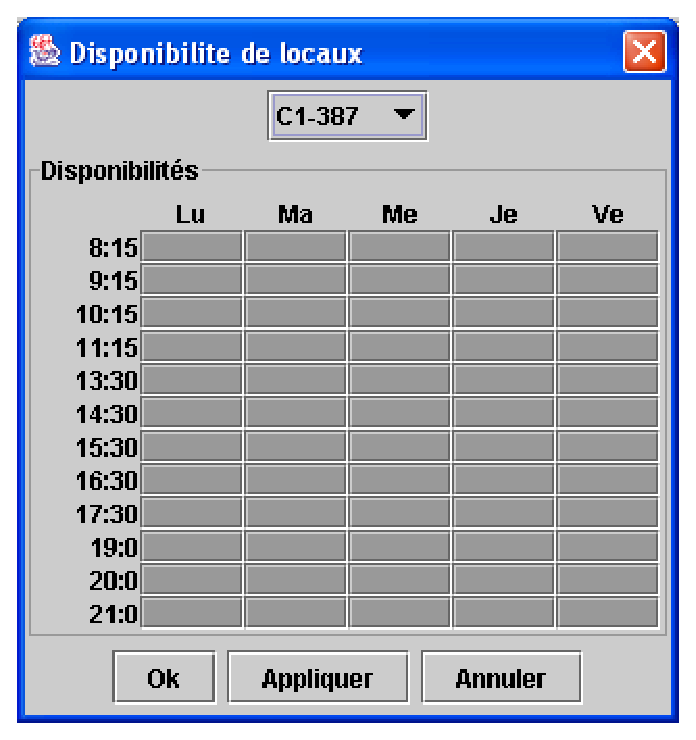
\includegraphics[width=2.5in]{UserManualInputs/images/local.eps}
        \caption{Disponibilit� des locaux}\label{localc}
      \end{center}
    \end{figure}

Cliquer sur \textbf{\emph{Appliquer}} pour accepter et effectuer les changements et Cliquer sur \textbf{\emph{Ok}} pour accepter, effectuer les changements et fermer la fen�tre.\\
        
 \end{itemize}    

\subsection{Construction de l'horaire}

\subsubsection{Affectation des �v�nements}

Il est vivement recommand� de commencer cette �tape en lan�ant l'\textbf{\emph{affectation initiale}} � partir du menu \textbf{\emph{Optimisation}} (si cela n'a pas �t� pr�c�demment fait � la fin de la phase de pr�paration de l'horaire - section \ref{finprepa}) avant de poursuivre la production de l'horaire.

L'\emph{affectation initiale} a pour but d'ex�cuter les commandes suivantes :

\begin{enumerate}
    \item Placer de fa�on al�atoire dans les groupes d'activit�, les �tudiants non pr�-affect�s � des groupes, tout en �quilibrant les groupes.
    \item Placer les �v�nements pr�-affect�s (plac�s ou fig�s) dans la grille horaire.
    \item Calculer les conflits g�n�r�s.
\end{enumerate}  

Une fois l'affectation initiale effectu�e, l'�tape suivante consiste � lancer le sous menu \textbf{\emph{Construire l'horaire}} � partir du menu \textbf{\emph{Optimisation}}, afin de laisser le logiciel placer automatiquement dans la grille horaire les �v�nements (ceux qui n'ont pas encore �t� plac�s dans la grille horaire) respectant toutes les contraintes sp�cifi�es et ne cr�ant aucun nouveau conflit (conflits d'enseignants, conflits d'�tudiants et conflits de locaux).

\subsubsection{Raffinement de l'horaire}


\section{Production d'un horaire d'examen}

\subsection{Pr�paration de l'horaire}\label{finprepae}

\begin{enumerate}
    \item Lancer \dx{}.
    \item Aller au menu \textbf{\emph{Fichier}},
    puis s�lectionner le menu \textbf{\emph{Nouvel horaire}}
    et enfin s�lectionner le sous-menu \textbf{\emph{Horaire Examen}}.
    Une bo�te de dialogue comme celle
de la Figure \ref{selectgrillecyc} doit appara�tre et elle vous
permettra de choisir le fichier (fichier avec extension \emph{.xml})
contenant la d�finition de votre grille horaire.

    \item En cliquant sur le bouton \emph{\textbf{OK}}, la grille horaire s�lectionn�e est charg�e et pr�sent�e � l'�cran (voir figure \ref{grilleexam}).
\begin{figure}[h]
  % Requires \usepackage{graphicx}
  \begin{center}
    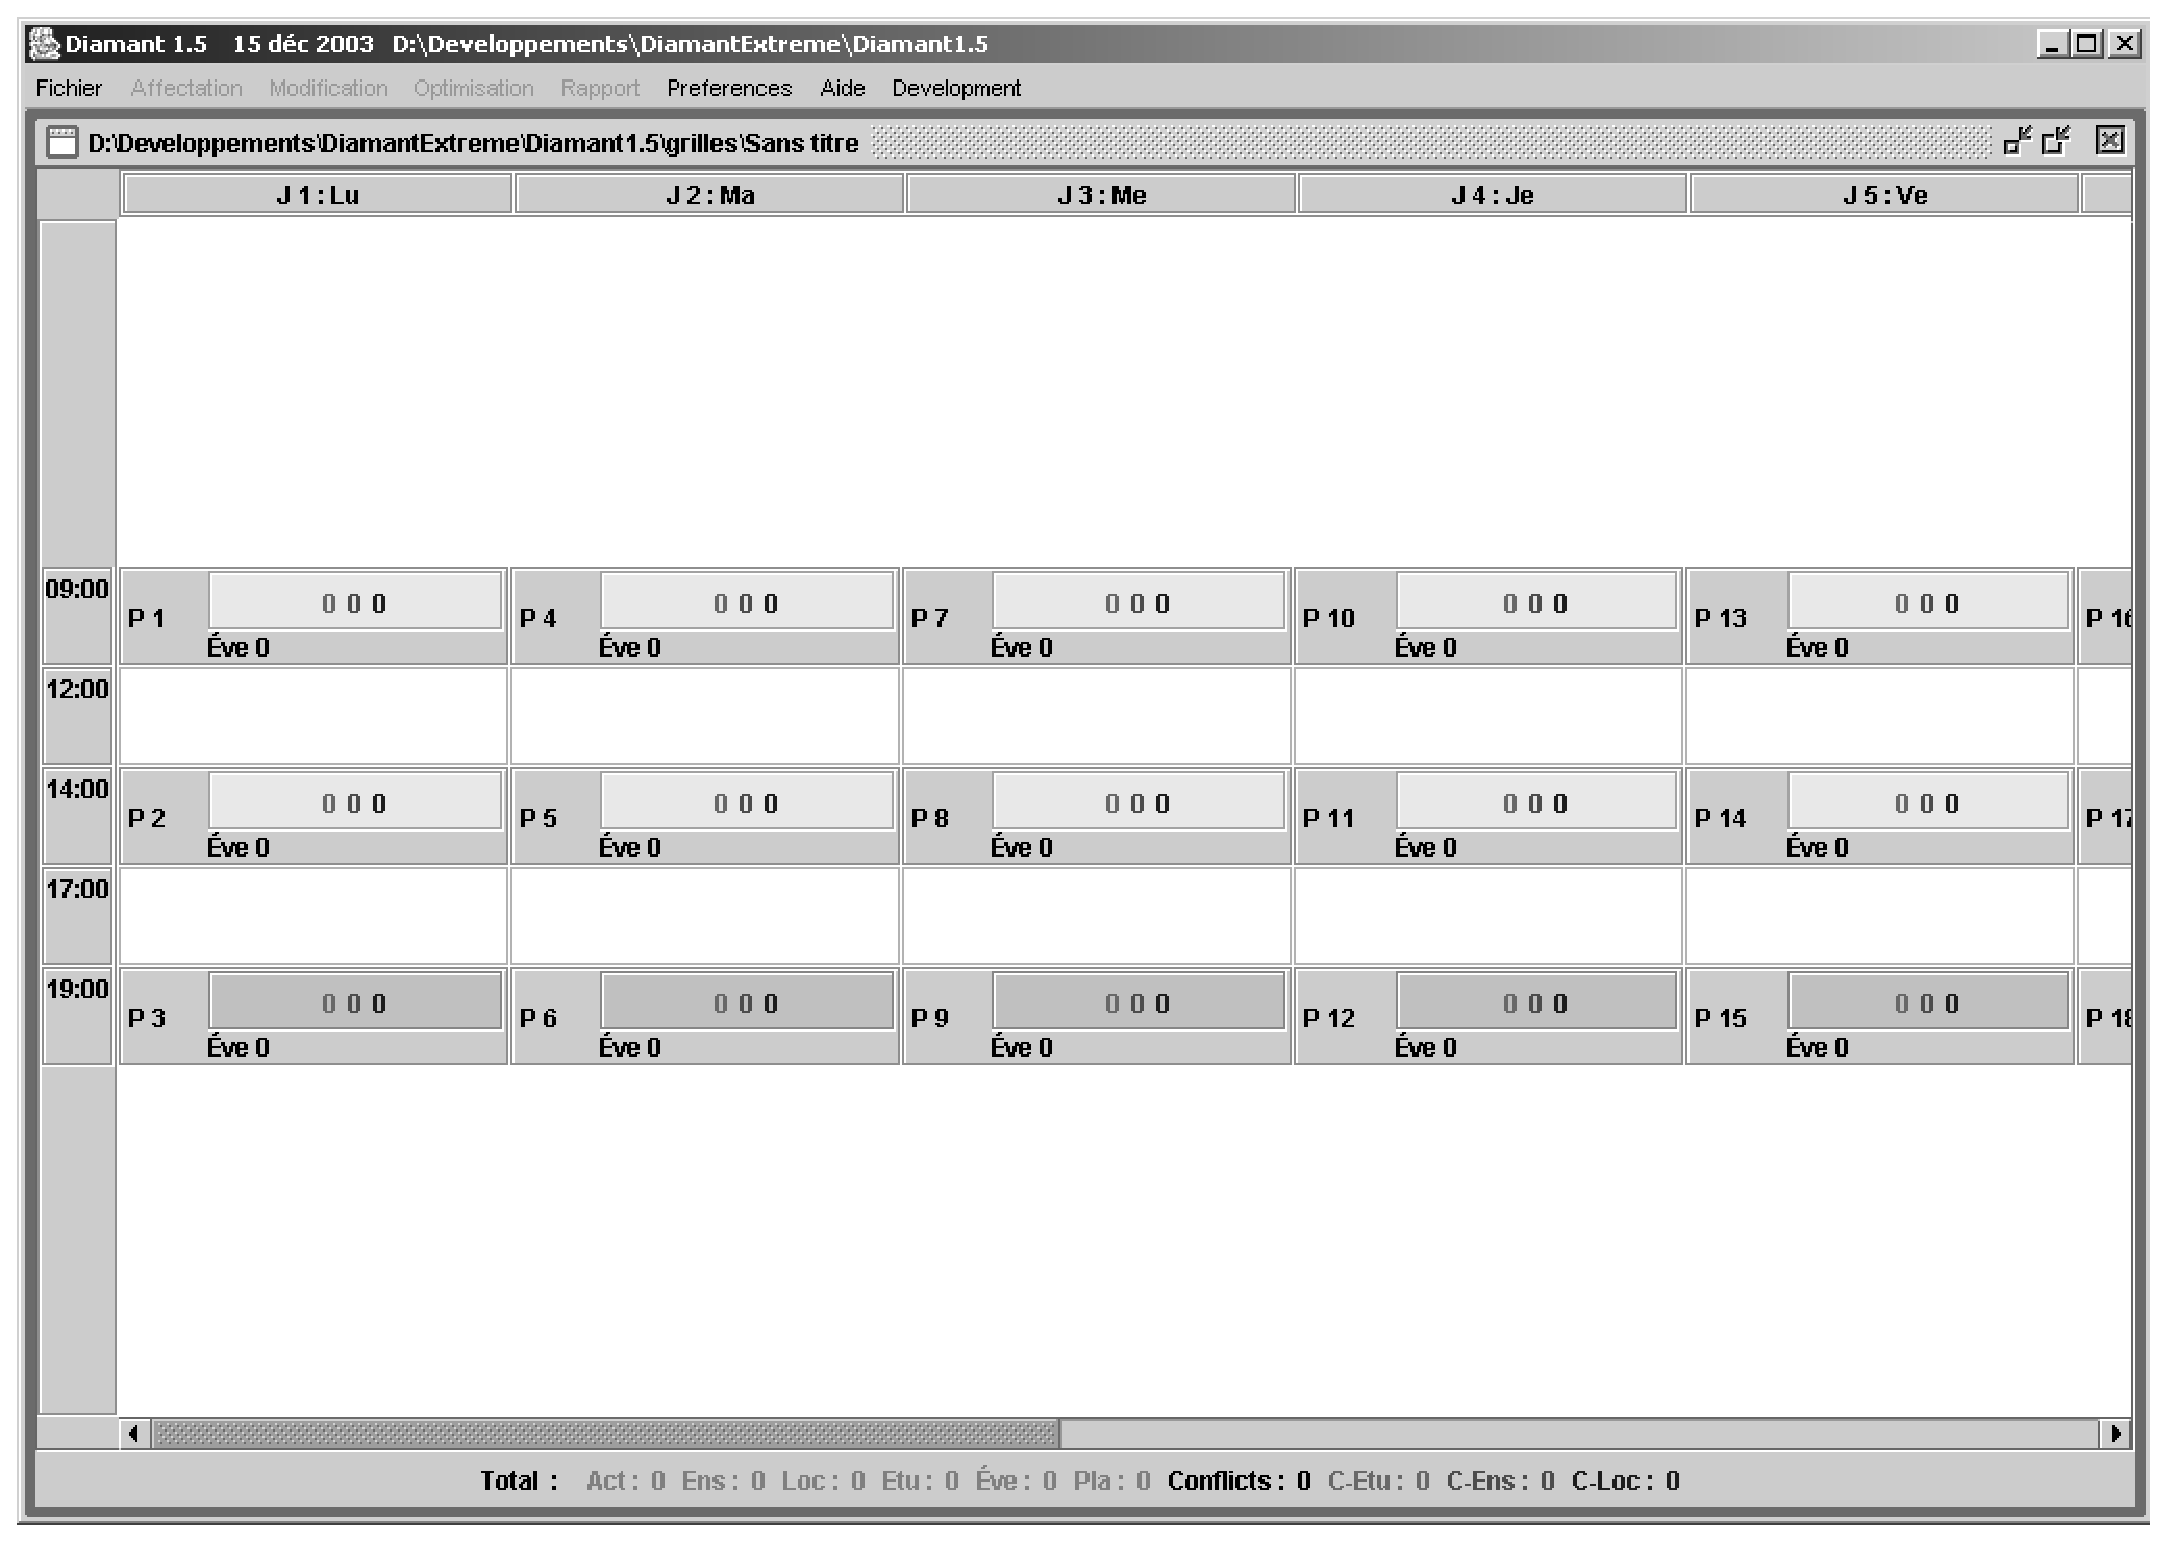
\includegraphics[width=4.5in]{UserManualInputs/images/grilleexam.eps}
    \caption{Grille horaire d'examen}\label{grilleexam}
  \end{center}
\end{figure}

    \item Aller au menu \textbf{\emph{Fichier}} et s�lectionner le menu \textbf{\emph{D�finir fichiers � importer}}. Une bo�te de dialogue comme celle de la Figure \ref{defautoimport}  doit appara�tre. Rep�rer l'endroit o� chacun des fichiers est localis�, puis cliquer sur le bouton \textbf{\emph{OK}}. Une nouvelle fen�tre se pr�sentera afin de vous permettre d'enregistrer la configuration des fichiers que vous venez de faire.

Il est recommand� d'enregistrer cette configuration en utilisant un nom de fichier unique et repr�sentatif.

Exemple: choisissez le nom de fichier \emph{H04exam} pour \emph{Hiver 2004 horaire d'examen} et le fichier cr�� sera \emph{H04exam.dim}. L'extension \textbf{\emph{.dim}} est rajout� automatiquement.

    \item Aller au menu \textbf{\emph{Fichier}} et s�lectionner le menu \textbf{\emph{Importer automatiquement}}.
    Une boite de dialogue appara�tra et vous permettra de choisir le fichier \textbf{\emph{.dim}} de �configuration de fichiers�
    pr�c�demment cr�� � partir de la fonction  \textbf{\emph{D�finir fichiers � importer}}
    (dans l'exemple pr�c�dent il s'agit du fichier \emph{H04exam.dim}).
    Cliquer � pr�sent sur le bouton \textbf{\emph{Importation de fichiers}},
    toutes vos donn�es (cours, �tudiants, enseignants et locaux) seront charg�es dans le logiciel et
    pr�tes � �tre modifi�es.
\end{enumerate}

� partir de cette �tape, la construction de l'horaire � proprement parler peut commencer. Il est vivement recommand� de lancer l'\textbf{\emph{Affectation initiale}} � partir du menu \textbf{\emph{Optimisation}} avant de poursuivre la production de l'horaire. Lancer l'\textbf{\emph{Affectation initiale}} � cette �tape ex�cuterait les fonctionnalit�s suivantes:

\begin{enumerate}
    \item Suppression des activit�s de nature 2, seulement les activit�s de nature 1 seront conserv�es pour l'horaire.
    \item Suppression des groupes aux activit�s en poss�dant plusieurs, un seul groupe sera conserv� pour l'horaire (le premier groupe ou \emph{groupe A}).
    \item Suppression des �v�nements aux activit�s en poss�dant plusieurs, un seul �v�nement sera conserv� pour l'horaire.
    \item Modification de la disponibilit� des enseignants afin de les rendre tous disponibles.
    \item Modification de la disponibilit� des locaux afin de les rendre tous disponibles.
\end{enumerate}

Exemple: Pour construire l'horaire d'examen d'une activit� (GEI200) poss�dant 2 natures (GEI200.1 et GEI200.2), chaque nature poss�dant 2 groupes (GEI200.1.A, GEI200.1.B et GEI200.2.A, GEI200.2.B), chaque groupe poss�dant 2 �v�nements (GEI200.1.A.1, GEI200.1.A.2, GEI200.1.B.1, GEI200.1.B.2 et GEI200.2.A.1, GEI200.2.A.2, GEI200.2.B.1, GEI200.2.B.2). La suppression de nature 2, de groupes et d'�v�nements par l'affectation initiale permettrait d'obtenir, pour l'activit� GEI200, un seul �v�nement devant servir � l'horaire d'examen, en l'occurrence GEI200.1.A.1.

Cette affectation initiale permettrait donc d'�purer les donn�es et d'initialiser le logiciel de sorte � pouvoir faire des modifications sur les donn�es et observer imm�diatement les repercussions sur l'horaire.

La pr�paration de l'horaire �tant achev�e, nous pouvons � pr�sent passer � la phase de modification et d'�puration de donn�es (phase 2). Il est cependant n�cessaire de noter que cette phase peut avoir lieu avant ou apr�s la phase de construction � proprement parler (phase 3), mais nous recommandons de la faire avant la phase 3 afin de travailler une bonne fois pour toute sur des donn�es propres (�pur�es).

\subsection{Modification et �purations des donn�es}

Le but de cette �tape est de permettre de construire l'horaire uniquement � partir de donn�es propres. Cette modification et/ou �puration peut se faire sur les activit�s, les �v�nements, les groupes d'�tudiants, les enseignants ou les locaux. 

\begin{itemize}
    \item Modifier une activit� en cliquant sur le menu \textbf{\emph{Affectation}} et le sous menu \textbf{\emph{Activit�s}} pour voir appara�tre la \emph{liste des activit�s} (voir figure \ref{listacte}) ou alors cliquer sur le menu \textbf{\emph{Affectation}} et le sous menu \textbf{\emph{�v�nements}} pour voir appara�tre la \emph{liste des �v�nements} (voir figure \ref{listeevente}).\\

� partir de la fen�tre \emph{liste des �v�nements}, vous pouvez s�lectionner un ou plusieurs �v�nements et les faire passer de la colonne \emph{fig�s} (les �v�nements sont plac�es et fig�es dans la grille horaire) � \emph{plac�s} (les �v�nements sont plac�es dans la grille horaire) ou de la colonne \emph{plac�s} � \emph{non plac�s} (les �v�nements ne sont pas encore plac�es dans la grille horaire) et vice-versa. 

    \begin{figure}[h]
      % Requires \usepackage{graphicx}
      \begin{center}
        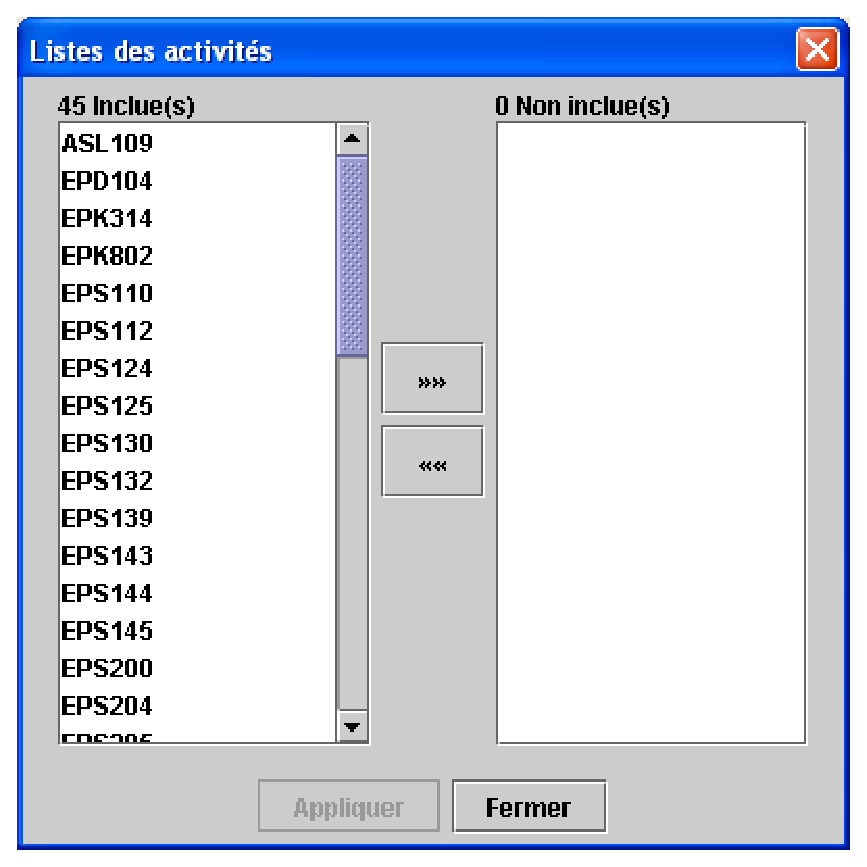
\includegraphics[width=2.5in]{UserManualInputs/images/listeact.eps}
        \caption{Liste des activit�s}\label{listacte}
      \end{center}
    \end{figure}

� partir de la fen�tre \emph{liste des activit�s}, vous pouvez s�lectionner une ou plusieurs activit�s et les faire passer de la colonne \emph{inclue(s)} � \emph{non inclue(s)} (non inclue(s)= les activit�s ne seront pas utilis�es dans la construction de l'horaire) et vice-versa. \\

    \begin{figure}[h]
      % Requires \usepackage{graphicx}
      \begin{center}
        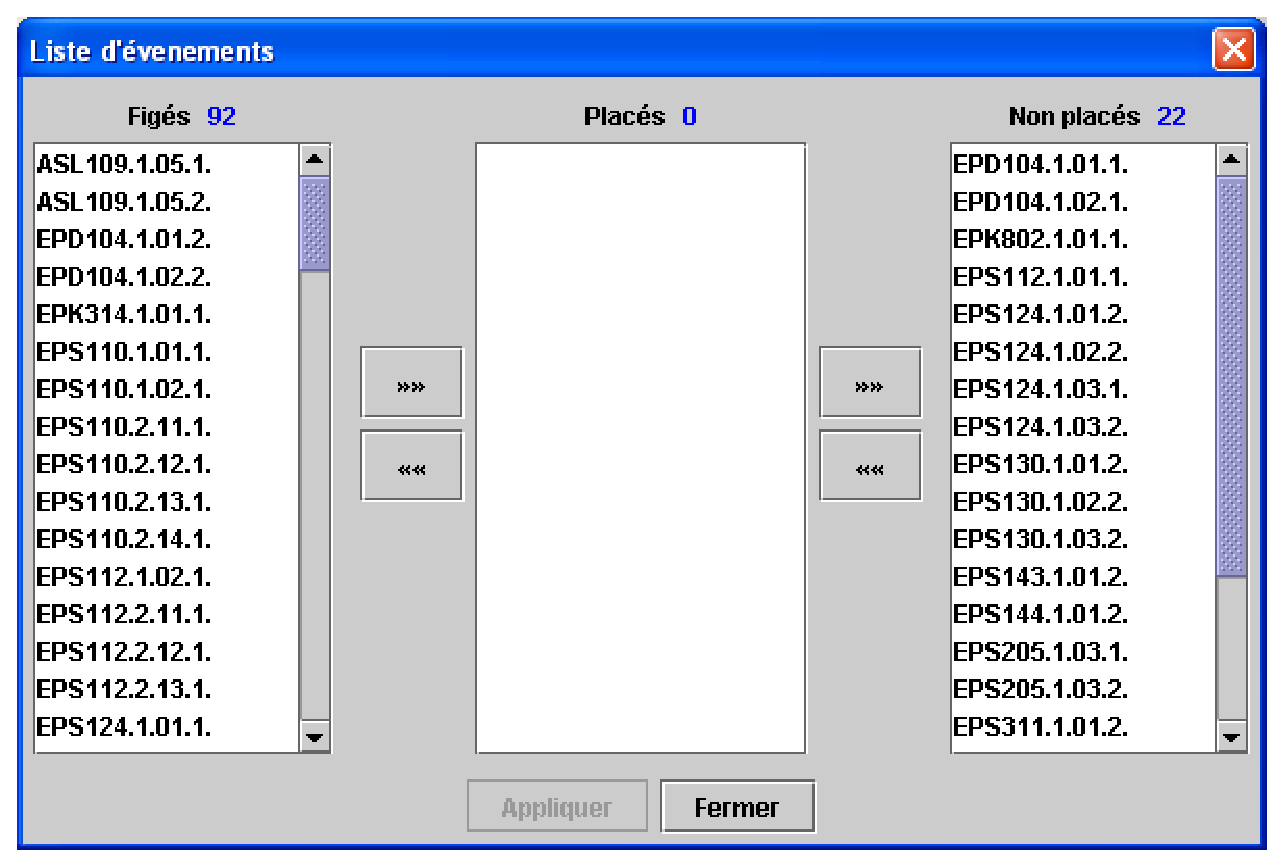
\includegraphics[width=2.5in]{UserManualInputs/images/listeevent.eps}
        \caption{Liste des �v�nements}\label{listeevente}
      \end{center}
    \end{figure}
   

� partir de l'une ou l'autre des fen�tres, double-cliquer sur l'activit� ou l'�v�nement � modifier pour faire appara�tre le dialogue d'\emph{affectation d'�v�nements} (voir figure \ref{evente}). Il vous est possible de modifier, � partir de cette fen�tre d'\emph{affectation d'�v�nements}, le jour et l'heure de d�but de l'�v�nement, l'enseignant, le local, de placer ou figer l'�v�nement.

    \begin{figure}[h]
      % Requires \usepackage{graphicx}
      \begin{center}
        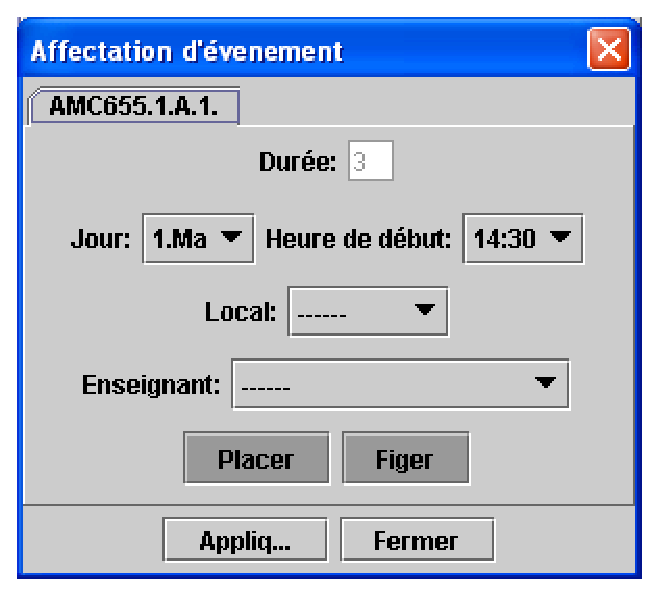
\includegraphics[width=2.5in]{UserManualInputs/images/event.eps}
        \caption{Affectation d'�v�nement}\label{evente}
      \end{center}
    \end{figure}
    
Cliquer sur \textbf{\emph{Appliquer}} pour valider les changements et Cliquer sur \textbf{\emph{Fermer}} pour fermer la fen�tre.\\
    
\item Modifier la disponibilit� d'un enseignant en cliquant sur le menu \textbf{\emph{Affectation}} et le sous menu \textbf{\emph{Enseignants}} pour voir appara�tre la fen�tre de la figure \ref{enseignante}. En s�lectionnant une zone correspondant au jour et � l'heure que vous souhaitez modifier. Une zone s�lectionn�e appara�t en fonc� et indique que l'enseignant y est disponible.
 
    \begin{figure}[h]
      % Requires \usepackage{graphicx}
      \begin{center}
        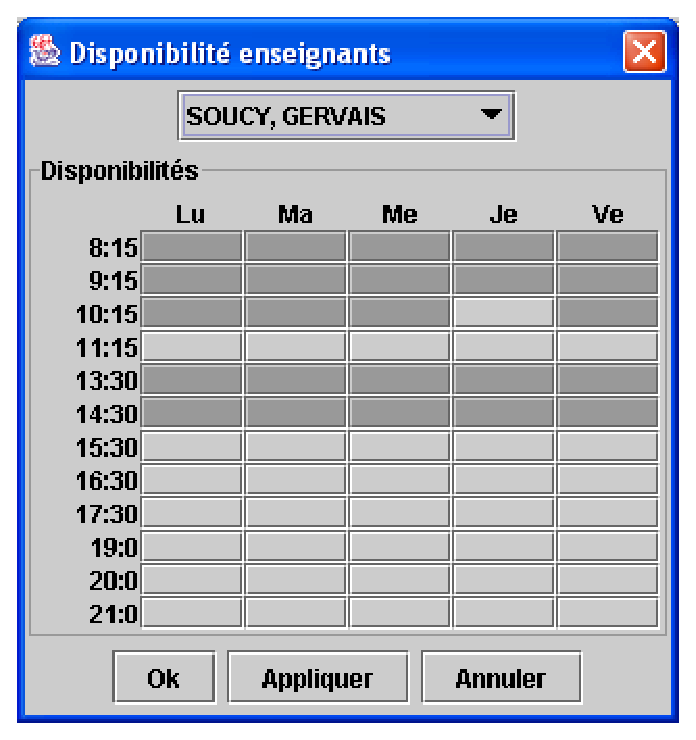
\includegraphics[width=2.5in]{UserManualInputs/images/enseignant.eps}
        \caption{Disponibilit� des enseignants}\label{enseignante}
      \end{center}
    \end{figure}

Cliquer sur \textbf{\emph{Appliquer}} pour accepter et effectuer les changements et Cliquer sur \textbf{\emph{Ok}} pour accepter, effectuer les changements et fermer la fen�tre.    \\

    \item Modifier la disponibilit� d'un local en cliquant sur le menu \textbf{\emph{Affectation}} et le sous menu \textbf{\emph{Locaux}} pour voir appara�tre la fen�tre de la figure  \ref{locale}. En s�lectionnant une zone correspondant au jour et � l'heure que vous souhait� modifier. Une zone s�lectionn�e appara�t en fonc� et indique que le local y est disponible. 

    \begin{figure}[h]
      % Requires \usepackage{graphicx}
      \begin{center}
        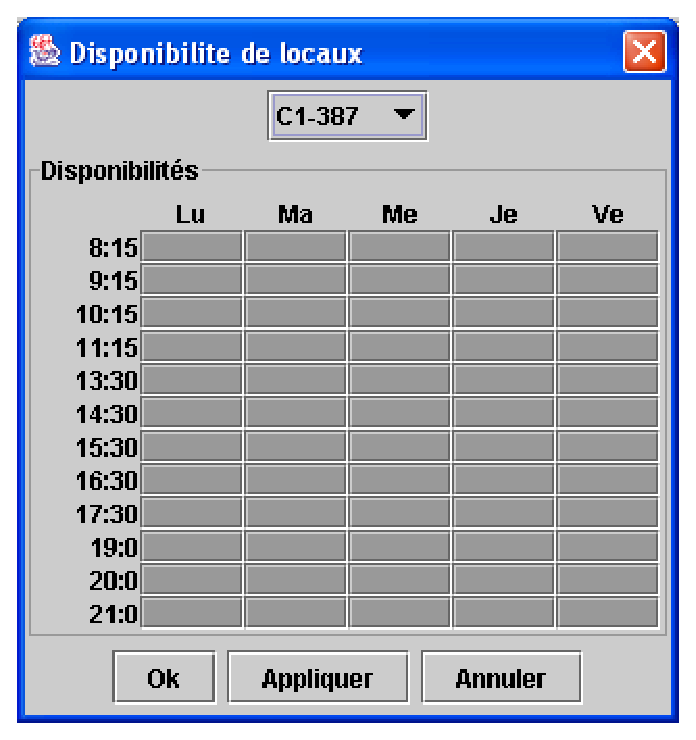
\includegraphics[width=2.5in]{UserManualInputs/images/local.eps}
        \caption{Disponibilit� des locaux}\label{locale}
      \end{center}
    \end{figure}

Cliquer sur \textbf{\emph{Appliquer}} pour accepter et effectuer les changements et Cliquer sur \textbf{\emph{Ok}} pour accepter, effectuer les changements et fermer la fen�tre.\\
        
 \end{itemize}    

\subsection{Construction de l'horaire}

Il est vivement recommand� de commencer cette �tape en lan�ant l'\textbf{\emph{affectation initiale}} � partir du menu \textbf{\emph{Optimisation}} (si cela n'a pas �t� pr�c�demment fait � la fin de la phase de pr�paration de l'horaire - section \ref{finprepae}) avant de poursuivre la production de l'horaire. La description des commandes ex�cut�es par l'affectation manuelle est faite � la section \ref{finprepae}.

Une fois l'affectation initiale effectu�e, l'�tape suivante consiste � lancer le sous menu \textbf{\emph{Construire l'horaire}} � partir du menu \textbf{\emph{Optimisation}}, afin de laisser le logiciel placer automatiquement dans la grille horaire les �v�nements (ceux qui n'ont pas encore �t� plac�s dans la grille horaire) respectant toutes les contraintes sp�cifi�es et ne cr�ant aucun nouveau conflit (conflits d'enseignants, conflits d'�tudiants et conflits de locaux).

La modification des contraintes � respecter par \dx{} lors de la construction automatique de l'horaire se fait en lan�ant le sous-menu \textbf{\emph{Options Conflits}} � partir du menu \textbf{\emph{Pr�f�rences}} pour faire appara�tre la fen�tre d'option de conflits (voir figure \ref{conf}). Cette fen�tre permet de modifier plusieurs param�tres, � savoir:

\begin{figure}[h]
      % Requires \usepackage{graphicx}
      \begin{center}
        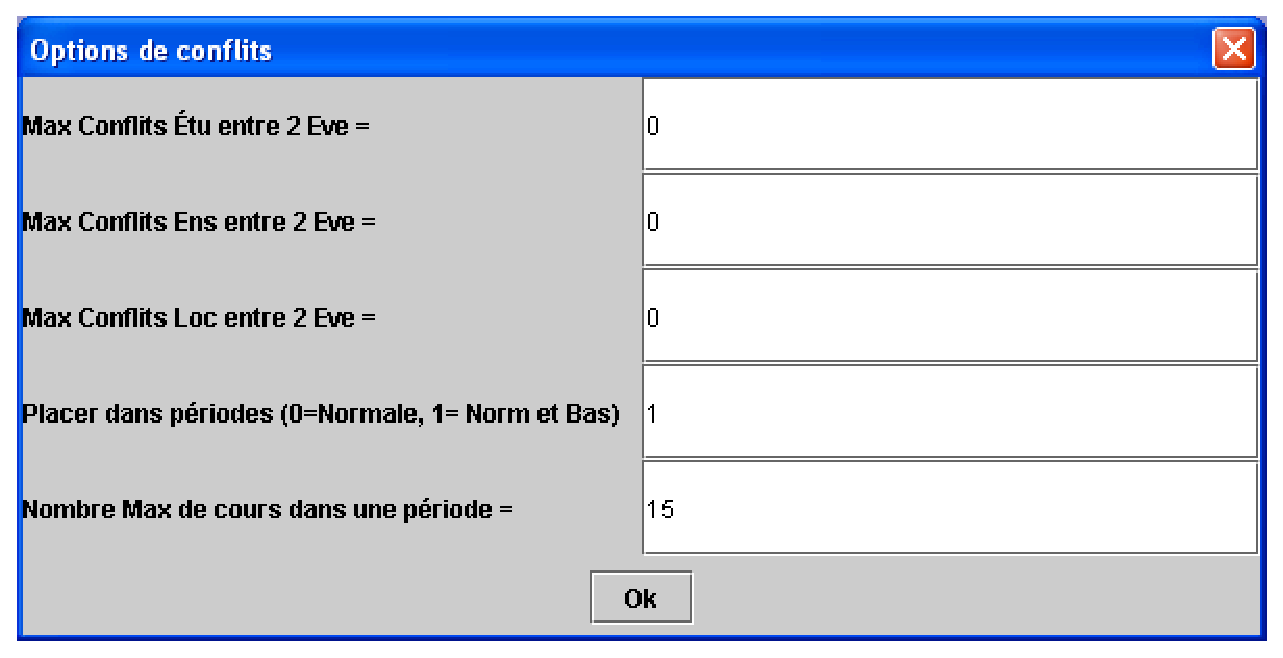
\includegraphics[width=3.5in]{UserManualInputs/images/optionconflict.eps}
        \caption{Contraintes � respecter}\label{conf}
      \end{center}
    \end{figure}

\begin{itemize}
    \item \emph{Max Conflits �tu entre 2 Eve}: ce param�tre permet de fixer le nombre maximal de conflits d'�tudiants admissible entre deux �v�nements.
    \item \emph{Max Conflits Ens entre 2 Eve}: ce param�tre permet de fixer le nombre maximal de conflits d'enseignants admissible entre deux �v�nements.
    \item \emph{Max Conflits Loc entre 2 Eve}: ce param�tre permet de fixer le nombre maximal de conflits de locaux admissible entre deux �v�nements.
    \item \emph{Placer dans p�riodes (0=normale, 1=normale et basse, 2=normale, basse et nulle)}: ce param�tre permet de sp�cifier les types de p�riodes (normale, basse, nulle) de la grille horaire dans lesquels un �v�nement peut �tre plac�.
    \item \emph{Nombre Max de cours dans une p�riode}: ce param�tre permet de sp�cifier le nombre maximal d'�v�nements pouvant �tre plac�s dans une m�me p�riode de la grille horaire.
\end{itemize}    

Il est possible de modifier les contraintes et lancer ensuite la construction de l'horaire afin que le logiciel  utilise les nouvelles contraintes pour placer les �v�nements qu'il n'a pas pu pr�c�demment placer; tout ceci de fa�on it�rative jusqu'� obtention d'un r�sultat paraissant satisfaisant aux yeux de l'utilisateur.

Si malgr� les it�rations, l'horaire construit n'est pas satisfaisant, il existe un certain nombre d'outils permettant de raffiner manuellement l'horaire.

\section{Raffinement de l'horaire}
Le raffinement de l'horaire propose � travers certains outils (affectation manuelle, rapport), les voies et moyens d'am�lioration de l'horaire construit.

\subsection{Affectation manuelle}

L'affectation manuelle permet � l'utilisateur de placer individuellement les �v�nements dans la grille horaire. Elle se fait � partir de la fen�tre d'\textbf{\emph{Affection manuelle}} (voir figure \ref{man}) obtenue � partir du sous-menu \textbf{\emph{Affectation manuelle}} du menu \textbf{\emph{Affectation}}.

    \begin{figure}[h]
      % Requires \usepackage{graphicx}
      \begin{center}
        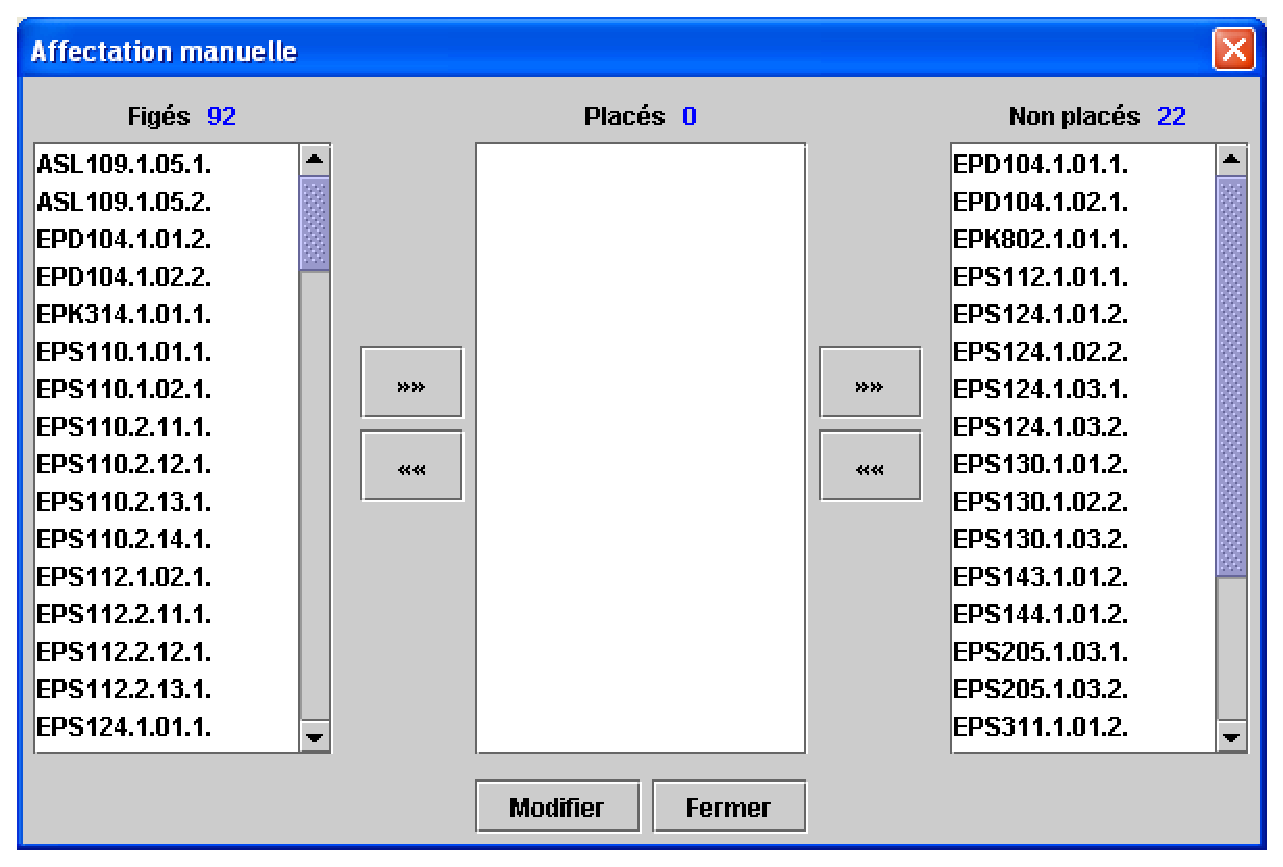
\includegraphics[width=3.5in]{UserManualInputs/images/manualaffect.eps}
        \caption{Liste des �v�nements}\label{man}
      \end{center}
    \end{figure}

La fen�tre d'affectation manuelle offre deux possibilit�s d'utilisation:

\begin{enumerate}
    \item \textbf{Modification d'un �v�nement:} s�lectionner un �v�nement et cliquer sur le bouton \textbf{\emph{Modifier}} pour faire appara�tre le dialogue d'\emph{affectation d'�v�nements} (voir figure \ref{evente}). Il vous est possible de modifier, � partir de cette fen�tre d'\emph{affectation d'�v�nements}, le jour et l'heure de d�but de l'�v�nement, l'enseignant, le local, de placer ou figer l'�v�nement.
    \item \textbf{Recherche de potentiels conflits:} pour rechercher les potentiels conflits g�n�r�s par un �v�nement, double-cliquer sur l'�v�nement en question pour voir appara�tre une nouvelle grille horaire (voir figure \ref{man1}) vous informant sur les conflits que peut g�n�r� l'�v�nement dans chaque p�riode de la grille horaire. \\

Une repr�sentation par les couleurs, de la grille horaire d'affectation manuelle, a �t� adopt�e afin de vous permettre, d'un seul coup d'oeil, de rep�rer les p�riodes de potentiels conflits (couleur rouge), les p�riodes dans lesquelles l'�v�nement peut �tre plac� sans g�n�rer de conflits (couleur par d�faut de la p�riode), et la ou les p�riodes dans lesquelles l'�v�nement est plac� (s'il �tait pr�c�demment plac� dans le grille - couleur verte).

    \begin{figure}[h]
      % Requires \usepackage{graphicx}
      \begin{center}
        \includegraphics[width=4.0in]{UserManualInputs/images/manualaffectres.eps}
        \caption{Grille horaire d'affectation manuelle}\label{man1}
      \end{center}
    \end{figure}

\end{enumerate}    

\subsection{Rapports}

\chapter{Description des menus, des dialogues et des fen�tres}

\section{DESCRIPTION DES MENUS}


\begin{description}
    \item[Fichier :] permet de faire appel aux fonctions classiques relatives aux fichiers : Nouveau
projet, Nouveau, Ouvrir, Fermer, Enregistrer, Enregistrer sous, Importer manuellement,
D�finir le fichier Import Auto, Importer automatiquement, Exporter et Quitter.
    \item[Affichage :] permet de faire appel aux fonctions n�cessaire � l'affichage des fen�tres associ�es � un projet d'horaire.
    \item[Affectation :] permet d'affecter (fixer) certains choix relatifs � la construction d'un horaire, par exemple, un �tudiant dans un groupe donn� ou une activit� � une p�riode d�termin�e, etc. Contient aussi les menus qui permettent la construction automatique optimis�e d'un horaire.
    \item[Rapport :] permet de faire appel aux fonctions qui donnent acc�s aux rapports et de les sauvegarder comme des fichiers � texte �.
    \item[Pr�f�rences :] permet le changement de certains param�tres du programme.
    \item[Fen�tre :] Permet d'ouvrir une fen�tre de listes de conflits pr�c�demment ouverte.
    \item[Aide :] permet d'obtenir de l'information sur le logiciel ainsi que de l'aide.
\end{description}    
 

%  
% 
% 
% 
% 

%\part{Une partie}
%\include{revue}
%\include{theorie}

%\part{Derni�re partie}
%\chapter{Conclusion}

Bla bla bla bla bla.

Bla bla bla bla bla.

%\chapter*{Glossaire}

Bla bla bla bla bla.

Bla bla bla bla bla.

%\chapter*{Index}

A
AAA
ABC.

B
Bla bla bla bla bla.

%\include{formules}
\end{articleDX}
\end{document}
